\documentclass[twocolumn,a4j,dvipdfmx]{jsarticle_customized1}

\usepackage{amssymb,amsmath,bm}
\usepackage{graphicx,tabularx}
\usepackage{times,type1cm}
\usepackage{url}
% \usepackage{fancyhdr}

\usepackage[
	sorting=none,
	isbn=false,
	doi=false,
]{biblatex}
\usepackage{color}
\addbibresource{references.bib}
\renewcommand{\bibfont}{\fontsize{7.5pt}{8.5pt}\selectfont}
\newcommand{\modify}[1]{{\color{red} #1}}


\author{橋本　良真}
\labname{情報メディア環境学研究室}
\title{スタイル変換を用いた画像合成のための領域分割による抽象度調整}

% \pagestyle{fancy}
% \lhead{}
% \chead{}
% \rhead{(1)A\textcircled{\scriptsize 1}}
% \cfoot{}

\begin{document}
\twocolumn[\maketitle \vspace{0.0zw}]

\setlength{\baselineskip}{13.2pt}
\setlength{\abovecaptionskip}{0pt}
\setlength{\belowcaptionskip}{-5pt}
% \setlength{\intextsep}{5pt}

\section{はじめに}\label{sec:introduction}
近年，イラストレーションや漫画に用いられる背景を写真やCGを用いることで効率的に制作する手法が頻繁に利用されており，その中でも写真を編集することで漫画調の背景とする利用方法は増加傾向にある．
しかし，既存の画像処理アプリケーションを用いた写真の編集は色調補正に関する専門的な知識を必要とすることに加え，彩度調整やコントラスト調整といった複数の補正操作を組み合わせなければならず，手間がかかる．
%そのため，目的の表現を実現するためにはそれらのパラメータを適切に選択しなければならず，手作業でのパラメータ探索は非常に手間がかかる．
そこで，画像のスタイル（雰囲気）を簡単に変換することのできるスタイル変換技術を用いて，背景として利用したい写真のスタイルを前景となるキャラクターなどのイラストのスタイルに変換することで，より効率的に背景画像を生成することができると考えられる．
しかし，この方法は絵画やパターン画像のスタイルを転送することには長けているものの，キャラクターなどのイラストに用いられる塗り方などの詳細なスタイルを転送する際には，全体への一律な処理によって不自然な色調の変化などの不具合が起こりやすい．
本研究では，画像のセグメンテーション（領域分割）や画像から計測される情報量を用いることで領域の情報量に応じた強度のスタイル変換処理を施し，変換後の画像の情報量が全体で一様となるように自然な変換画像を生成する手法を提案する．

\section{提案手法}\label{sec:proposed_method}
%提案手法の概要を図\ref{fig:method_overview}に示す．
本研究では，前景画像にとって自然な背景画像を生成するための二つの異なる手法を提案する．
\ref{sec:teian1}節では，領域ごとの情報量と前景画像の情報量に応じてスタイル変換のパラメータを決定する手法について紹介し，\ref{sec:teian2}節では，ユーザごとの好みを反映した画像を生成する目的のためパラメータの決定にベイズ最適化を用いる手法について紹介する．

%\begin{figure}[h]
%	\centering
%	\includegraphics[width=\linewidth]{．/figure/gaiyou．png}
%	\caption{提案手法の概要}
%	\label{fig:method_overview}
%\end{figure}

\subsection{画像の情報量を用いる手法}\label{sec:teian1}
本節では，画像の情報量を用いて変換パラメータを推定する手法について説明する．
この手法では，ユーザの操作によってスタイル変換に用いるコンテンツ画像を領域分割し，それぞれの領域における情報量を輪郭線割合と色相のエントロピーの二つの軸によって計算する．
これらの計算された情報量に基づいてスタイル変換のパラメータを決定することで，それぞれの領域に適した過不足のないスタイル変換を行い自然な生成画像を得る．
以下， 提案手法の具体的な流れについて述べる．

まず， 入力された背景画像をWatershedアルゴリズムにより領域分割する．
%Watershedアルゴリズムとは，画素の輝度値の極大値と極小値を用いた領域分割手法の一つである．
提案手法では，ユーザはインターフェースにより画像上の複数の位置にマーカーをヒントとして配置し，その情報をもとに画像を複数の領域に分割する．
次に， 変換パラメータを決定するため，入力された画像の情報量を計算する．
前景画像及び背景画像の情報量は，エントロピーと輪郭線割合の二つの情報から計算される．
エントロピーは画像の持つ色相のヒストグラムから計算される．色相は256段階に離散化されているものとして計算する．
画像の輪郭線割合はCannyフィルタによって抽出された輪郭線画像において，全画素のうち輪郭線を表す画素の割合を計算することで求まる．
最後に，画像の全体情報量をエントロピーと輪郭線割合の加重和として定義する．

画像の情報量を求めた後，その値からスタイル変換のパラメータ$\alpha$を各領域に対して以下のようなヒューリスティックな手法で決定する．
領域$i$に対して，そのパラメータ$\alpha_i$は次式により決定される．
\begin{equation}
    \alpha_i = 1.0 - q_f + D_i,
    \label{equ:alpha:1}
\end{equation}

ただし，
\begin{equation}
    \alpha_i = \begin{cases} 
    0 & \text{if } \alpha_i < 0 \\
    1 & \text{if } \alpha_i > 1
    \end{cases}
\end{equation}
とする．
ここで，$q_f$は前景画像の全体情報量である．
また，$D_i$は次式によって求められる．
\begin{equation}
D_i = 
\begin{cases}
 -0.2 & (0 \leq q_i < 0.6) \\
 0 & (0.6 \leq q_i < 0.8) \\
 0.2 & (0.8 \leq q_i \leq 1.0)
\end{cases},
\label{equ:alpha:2}
\end{equation}
ここで，$q_i$は領域$i$の全体情報量である．

全ての領域のスタイル変換が終了した後，それぞれの領域を乗算処理により合成することでスタイル変換画像が生成される．

\subsection{ベイズ最適化を用いる手法}\label{sec:teian2}
本節では，ブラックボックス関数の最適解を効率的に求める手法であるベイズ最適化を用いて，個人の好みを反映した画像生成をする方法について説明する．
%ベイズ最適化は最適化途中に得られる目的関数値の履歴から関数形を推定し，最も良い解が得られる可能性が高い解候補を探索する手法である．

提案手法では，ユーザインタフェースによる生成画像に対するユーザの評価によってベイズ最適化が進行する．
画像の評価はユーザインタフェースによって1点から10点の10段階で行われる．
%生成された画像が前景画像に適しているほど高い点数をつけることとする．
画像の評価が行われる度に，ベイズ最適化によって最適解となる可能性が最も高いパラメータの組み合わせが提案されるため，それらを用いた生成画像を表示し次の評価を待機する．
評価と生成を繰り返し，最終的にユーザが満足したタイミングで最適化を終了する．

図\ref{fig:ui}にユーザが画像生成を行う際に使用するユーザインタフェースを示す．
\textcircled{\scriptsize 1}には生成された画像が表示される．ユーザが画像を評価する度に，ベイズ最適化によって提案されたパラメータを用いた画像が自動で生成され表示される．
\textcircled{\scriptsize 2}にはガイドとしてコンテンツ画像が領域ごとに表示される．
\textcircled{\scriptsize 3}は画像の評価を行うボタン，前景画像の表示と非表示を切り替えるボタンが配置されている．

\begin{figure}[hbt]
	\begin{center}
		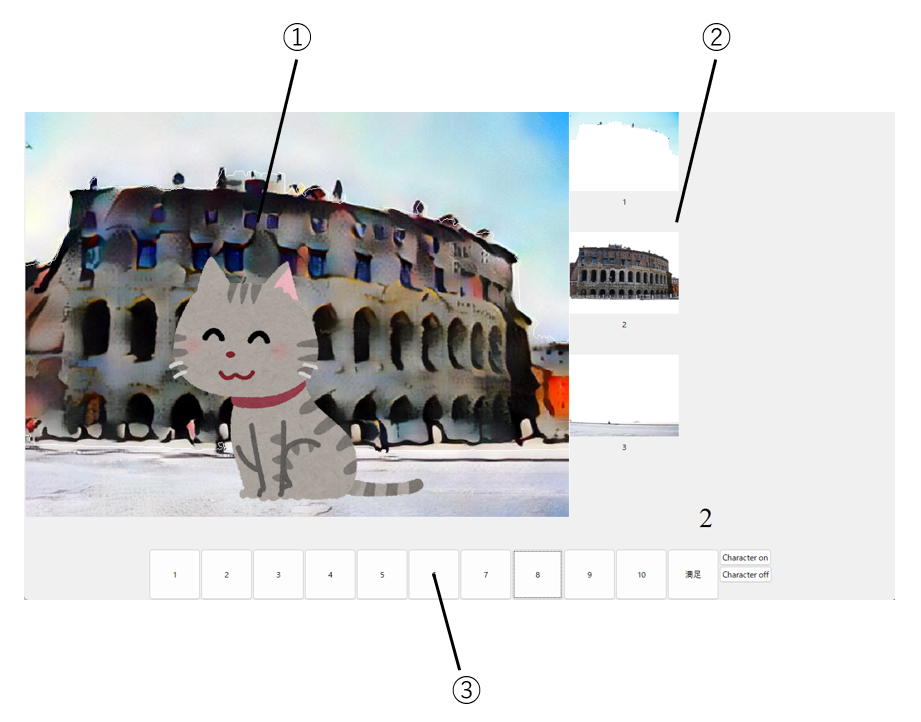
\includegraphics[width=0.9\linewidth]{./figure/ui.png}
	\end{center}
	\caption{ユーザーインターフェース}
	\label{fig:ui}	
\end{figure}

\section{実験結果}\label{sec:results}

提案手法によるスタイル変換の結果を示す．
本実験では，13th Gen Intel Core i7 13700(CPU)，32GBメモリ，NVIDIA GeForce RTX 4070 Ti(GPU)を搭載したWindows PCを用いた．
ただし，ユーザスタディではIntel Core i7 1065G7 CPU @ 1．30GHz，16GBメモリ，Intel Iris Plus Graphicsを搭載したWindows PCを用いた．

提案手法による生成画像例を図\ref{fig:result_info}に示す．
上段にスタイル変換に使用したコンテンツ画像とスタイル画像を示す．
中段に従来手法による生成画像を示す．
下段左に\ref{sec:teian1}節で述べた手法によってスタイル変換された生成画像を示す．また，下段右に\ref{sec:teian2}節で述べた手法による生成画像を示す．
従来手法でのスタイル変換では不自然な彩度の変化やエッジの強調が見られるが，提案手法でのスタイル変換ではそれらが抑制できたことが確認できる．

次に，\ref{sec:teian2}節で述べた手法の有効性を検証するため，ユーザスタディとして手動によるパラメータ調整との比較実験を行った．
9人の被験者にベイズ最適化によるパラメータ調整と手動によるパラメータ調整をそれぞれ2回ずつ行ってもらい，それぞれの調整で満足する画像が得られた人数と満足するまでにかかった時間を計測した．
表\ref{tab:userstudy_1}及び表\ref{tab:userstudy_2}に，ユーザスタディの結果を示す．
満足ボタンを押した人数については，領域数がいずれの場合もベイズ最適化による調整と手動による調整で大差は見られなかったが，満足ボタンを押すまでの平均時間はベイズ最適化による調整が手動による調整に比べて半分ほどに短縮されている．したがって，本UIが手動による探索と同等の探索性能を持ちつつ，探索の所要時間を大幅に短縮させることが確認できた．
3分間での画像の生成回数は，領域数が3つの場合はベイズ最適化による調整と手動による調整でほぼ同等だったが，領域数が5つの場合はベイズ最適化による調整が手動による調整と比べて約4回少なかった．これは領域数が増えるほどベイズ最適化におけるパラメータ推定に時間がかかるためで，領域数がさらに増加した場合は手動による調整がより効率よくパラメータ探索を行える可能性がある．

\begin{figure}[h]
	\centering
	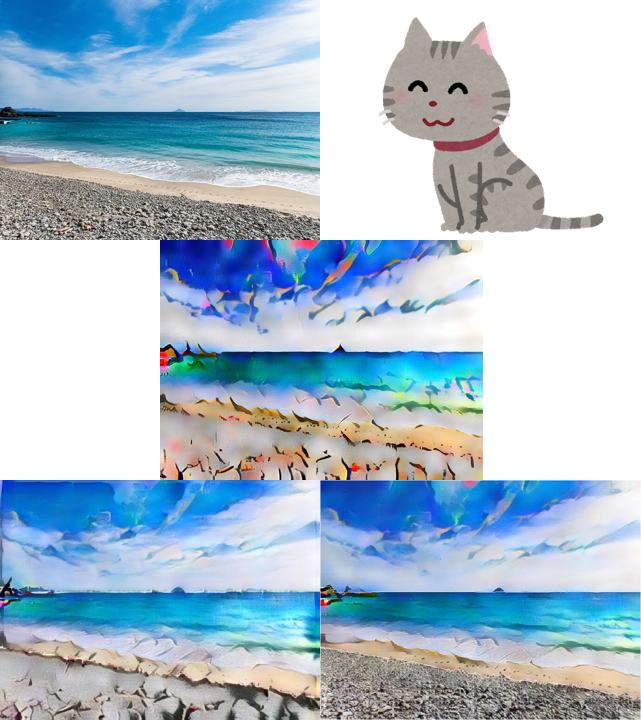
\includegraphics[width=\linewidth]{./figure/result.png}
	\caption{提案手法による生成画像例}
	\label{fig:result_info}
\end{figure}

\begin{table}[hbt] 
\vspace*{0.5mm}
\hbox to\hsize{\hfil
\begin{tabular}{l|c|c}
\hline
&ベイズ最適化&手動\\
\hline
満足ボタンを押した人数&6&7\\
\hline
満足するまでの平均時間(秒)&62.1&121.1\\
\hline
平均試行回数(回)&21.8&20.2\\
\hline
\end{tabular}\hfil}
\caption{3つに領域分割された背景画像を用いた\\
ユーザスタディの結果}
\label{tab:userstudy_1}
\end{table}

\begin{table}[hbt] 
\vspace*{0.5mm}
\hbox to\hsize{\hfil
\begin{tabular}{l|c|c}
\hline
&ベイズ最適化&手動\\
\hline
満足ボタンを押した人数&6&5\\
\hline
満足するまでの平均時間(秒)&71.5&151.6\\
\hline
平均試行回数(回)&14.4&18.4\\
\hline
\end{tabular}\hfil}
\caption{5つに領域分割された背景画像を用いた\\
ユーザスタディの結果} 
\label{tab:userstudy_2}
\end{table}

\section{まとめと今後の課題}\label{sec:summary}
本研究では，キャラクターイラストをスタイル画像，背景画像をコンテンツ画像としてスタイル変換を利用することで，キャラクターイラストに適した背景画像を効率的に生成する手法について紹介した．
コンテンツ画像を分割された領域ごとにスタイル変換することにより， 不自然な処理を抑制することが出来た．

今後の課題として， どちらの手法についても分割された領域の数が増えるほど処理時間が増加してしまうため，より高速な計算方法について考察する必要があると考えられる．また，どちらの手法についてもヒューリスティックな方法で手順や数値を決定している箇所があるため，より効果的な手法が存在するか検討することが必要である．

\printbibliography[title={参考文献}]

{\fontsize{7.5pt}{8.5pt}\selectfont\section*{\normalsize{\bf{著者の研究業績}}}
	\newcounter{number}
	\setcounter{number}{1}
	\newcommand{\num}{\arabic{number}}
	\begin{enumerate}
            \item[ [\num] \hspace{-0.8zw} ] \addtocounter{number}{1}
    	\underline{橋本 良真}, 土橋 宜典
    	``GANを用いた建物画像生成に関する一検討'',
    	電気・情報関係学会北海道支部連合大会 2021,
        (November. 2021).
    
            \item[ [\num] \hspace{-0.8zw} ] \addtocounter{number}{1}
    	\underline{Ryoma Hashimoto}, Yoshinori Dobashi
    	``Adjusting Level of Abstraction for Stylized Image Composition'',
    	SIGGRAPH Asia 2022,
        (December. 2022)．
    
            \item[ [\num] \hspace{-0.8zw} ] \addtocounter{number}{1}
    	\underline{Ryoma Hashimoto}, Yoshinori Dobashi
    	``Bayesian Optimization for Stylized Image Composition'',
    	NICOGRAPH International 2023,
        (June. 2023)．
    
	\end{enumerate}
}

\end{document}
